\documentclass[10pt]{article}
\usepackage{NotesTeX} %/Path/to/package should be replaced with package location
\usepackage{lipsum}
\usepackage{tensor}
\usepackage{amsmath,amsthm,amssymb}
\usepackage{hyperref}
\usepackage{tikz}
\usepackage{tikz-cd}
\tikzcdset{every label/.append style = {font = \small}}
\tikzcdset{row sep/normal=3.5em}
\tikzcdset{column sep/normal=3.5em}
\usetikzlibrary{shapes.geometric, arrows}

\usetikzlibrary{matrix}
\usetikzlibrary{decorations.markings,calc,shapes}
\usetikzlibrary{positioning}
\usepackage{graphicx}
\usepackage{empheq}
\usepackage{physics}
\usepackage{siunitx}
\usepackage{tensor}

\usepackage{multicol}

\newcommand{\bs}{\textbackslash}


\title{{\Huge General Relativity}\\{\Large{Class 31}}} %replace with class number
\author{Josephina Wright}

\emailAdd{jrwright@utexas.edu} %replace with your email
\begin{document}
    \maketitle
    \flushbottom
    \newpage
    \pagestyle{fancynotes}
    \part{Black Holes: Conformal Diagrams and Causality}
WORK IN PROGRESS!!!
\newline A black hole is set of events (an event defined as a point in the spacetime manifold) that can never communicate with asymptotic infinity. This means that regions in the manifold cannot communicate with regions that are arbitrarily far away. Communication is done by sending a causal cure, timelike or null, out to infinity. 
	The event horizon is the boundary of the black hole
              	\section{Conformal Transformations }\label{sec:class_style}
              		 A metric is conformally related to another metric if
              		 \begin{equation}
              		 \widetilde{g_{uv}}=\omega(x^u)^2g_(uv)
              		 \end{equation}
              		 Where \(\omega\) is a function of spacectime.  \(\omega\) is essentially re-scaling the proper times and proper distances in the spacetime in a position dependent manner. The resulting 	\(\widetilde{g_{uv}}\) is a conformal transform of guv.
              	\(\widetilde{g_{uv}}\) is oft4en viewed as unphysical, since guv solves Einstein's field equations for some sources, but 	\(\widetilde{g_{uv}}\) will not solves Einstein's field equations with those sources. 	\(\widetilde{g_{uv}}\) is not a physical metric, simply a tool that can be used to understand spacetime.
              		 For example, the Weyl tensor can be calculated with guv or 	\(\widetilde{g_{uv}}\), while both options are equal, they are noted by 
              		  \begin{equation}
              		\widetilde{C^u_{v\rho\sigma}}=C^u_{v\rho\sigma}
              		 \end{equation}
              		 Where the following is not equal to each other
              		   \begin{equation}
              		\widetilde{C_{uv\rho\sigma}}\neq{C_{uv\rho\sigma}}
              		 \end{equation}
              		 This is because the index is lowered using the 	\(\widetilde{g_{uv}}\) and guv respectively. In other words, 
              		  \begin{equation}
              	 \widetilde{g_{u\alpha}}\widetilde{C^\alpha_{v\rho\sigma}}\neq{g_{u\alpha}C^\alpha_{v\rho\sigma}}
              		 \end{equation}
              		  	Another fact that makes conformal transformations useful in understanding a metric that is physical is, given a null vector \(k^u\) (where \(k^uk^v\widetilde{g_{uv}}=0\)) Then \(k^u\) is null with respect to \(\widetilde{g_{uv}}\):
              		  		 \begin{equation}
              		 k^uk^v\widetilde{g_{uv}}=\omega(k^uk^vg_{ev})^2=0
              		 \end{equation}
              		 Conformal transformations preserve the light cone structure. If two events are related by a null trajectory in \({g_{uv}}\), then they are also connected by a null trajectory in 	\(\widetilde{g_{uv}}\). 
              		 
               	\section{Conformal Diagrams}\label{sec:class_style}
               	INSERT explanation here.
                                             \begin{figure}[!h]
               \centering
  \begin{tikzpicture}[x=0.75pt,y=0.75pt,yscale=-1,xscale=1]
  %uncomment if require: \path (0,163); %set diagram left start at 0, and has height of 163
  \tikzstyle{arrow} = [thick,->,>=stealth]
  %LEFT
 \draw [arrow] (-200,100) -- (-200,0);
  \draw[arrow]  (-200,100) -- (-100,100);
%RIGHT
 \draw [arrow] (0,100) -- (0,0);
  \draw [arrow] (0,50) -- (81.5,50);

%Light Cones
\draw (60,20) ellipse (10 and 2.5);
\draw (60,40) ellipse (10 and 2.5);
\draw (50,20)--(70,40)
\draw (70,20)--(50,40)



\draw (20,70) ellipse (10 and 2.5);
\draw (20,90) ellipse (10 and 2.5);
\draw (10,70)--(30,90)
\draw (30,70)--(10,90)
%Draw top arrow
\draw [arrow] (-120,-20) -- (-20,-20);

  % Label the points
  \draw  (91,40)node [anchor=north west][inner sep=0.75pt]    {$\widetilde{R}$};
  \draw (-15,0) node [anchor=north west][inner sep=0.75pt]    {$ \widetilde{T}$};

 \draw  (-90,100)node [anchor=north west][inner sep=0.75pt]    {r};
  \draw (-215,0) node [anchor=north west][inner sep=0.75pt]    {t};

  \draw  (-200,-30)node [anchor=north west][inner sep=0.75pt]    {$(t,r,\theta,\phi)$};
  \draw  (0,-30)node [anchor=north west][inner sep=0.75pt]    {$(\widetilde{T},\widetilde{R},\theta,\phi)$};
  
  \end{tikzpicture}
  \caption{Showing what a conformal diagram will do for our coordinates }
  \label{fig:lineup}
              \end{figure}  
               
               
               	The goal is to draw a spacetime diagram of all the spacetime, plus infinity. This is done by making a spacetime diagram of Equation 1.1
              Example: Minkowski Spacetime
              \begin{equation}
                  ds^2=-dt^2+dr^2+r^2d\Omega^2
              \end{equation}
              
              \begin{equation}
                  ds^2=\frac{1}{(cos{-\tilde{T}}+cos{\tilde{R})}^2}(d\tilde{T}+d\tilde{R}+sin(\tilde{R})^2d\omega^2)
              \end{equation}
              This is a conformal factor multiplied by a simple metric, so if the first term were to instead be written as $\omega$, a conformal factor, then
                            \begin{equation}
                                d\widetilde{s}^2=\omega^2ds^2=(-d\tilde{T}^2+d\tilde{R}^2+sin(\tilde{R})^2d\omega^2)
                            \end{equation}
                           The metric $d\widetilde{s}$ is a simpler metric that can now be drawn with a conformal diagram, with the restricted ranges of $|\widetilde{T}|+\widetilde{R}<\pi$. EXPLAIN T AND R CONSTANT SURFACES
                              \begin{figure}[!h]
               \centering
  \begin{tikzpicture}[x=0.75pt,y=0.75pt,yscale=-1,xscale=1]
  %uncomment if require: \path (0,163); %set diagram left start at 0, and has height of 163
  \tikzstyle{arrow} = [thick,->,>=stealth]
  %Draw the legend on the side
 \draw [arrow] (-120,81.5) -- (-120,40);
  \draw [arrow]  (-120,81.5) -- (-80,81.5);
%Draw triangles
 \draw[dashed] (0,0) -- (0,163);
 \draw (0,0) -- (150,81.5);
  \draw (0,163) -- (150,81.5);
 %Draw Vertical curves
 \draw (0,0) .. controls (20,74) and (20,89) .. (0,163);
  \draw (0,0) .. controls (60,74) and (60,89) .. (0,163);
   \draw (0,0) .. controls (100,74) and (100,89) .. (0,163);
   %Draw Horizontal curves
     \draw (0,81.5) -- (150,81.5);
   \draw (0,40) .. controls (60,40) and (100,60) .. (150,81.5);
 \draw (0,123) .. controls (60,123) and (100,103) .. (150,81.5);
  % Label the points
  \draw  (-80,81.5)node [anchor=north west][inner sep=0.75pt]    {$\widetilde{R}$};
  \draw (-120,20) node [anchor=north west][inner sep=0.75pt]    {$ \widetilde{T}$};
  
  \draw (0,-20) node [anchor=north west][inner sep=0.75pt]    {$\widetilde{R}=0, \widetilde{T}=\pi$};
   \draw (0,183) node [anchor=north west][inner sep=0.75pt]    {$\widetilde{R}=0, \widetilde{T}=-\pi$};
    \draw (163,81.5) node [anchor=north west][inner sep=0.75pt]    {$\widetilde{R}=\pi, \widetilde{T}=0$};
% Draw the points
\filldraw [black] (0,0) circle (2pt);
% Draw the points
\filldraw [black] (0,163) circle (2pt);
% Draw the points
\filldraw [black] (150,81.5) circle (2pt);
  \end{tikzpicture}
  \caption{Conformal Diagram of Minkowski Space: Restricted by $|\widetilde{T}|+\widetilde{R}<\pi$ }
  \label{fig:lineup}
              \end{figure}         
    \newline	Steps to derive conformal diagram for Minkowski
               	(Can be found in Appedix H of Carroll)
               	\begin{enumerate}
                    \item use null coordinates 
                    \begin{equation}
                   \begin{align}
                        u=t-r && v=t+r\\
                        t=\frac{v+u}{2} &&r=\frac{v-u}{2} \\
                        -\infty>u>\infty && -\infty>v>\infty\\
                        && v\geq{u}
                        \end{align}
                    \end{equation}
                    Where the \(v\geq{u}\) condition comes from the fact that r must be positive. 
                    In these coordinates, the metric can be written as 
                    \begin{equation}
                        ds^2=\frac{-1}{2}(dudv+dvdu)^2+r^2\Omega^2
                    \end{equation}
                    Remembering that \(dudv+dvdu=2dudv\)
                    \item Compactify coordinates
                    \begin{equation}
                   \begin{align}
                        u=tan(\widetilde{U}) && v=tan(\widetilde{V})\\
                        -\frac{\pi}{2}<tan(\widetilde{U})<\frac{\pi}{2} && -\frac{\pi}{2}<tan(\widetilde{V})<\frac{\pi}{2}
                        \end{align}
                    \end{equation}
            Now the coordinate system is such that whole metric can be written in a finite range of coordinates.
                                \begin{equation}
                   \begin{align}
                        du=sec^2(\widetilde{U}d\widetilde{U})&&dv=sec^2(\widetilde{V}d\widetilde{V})\\
                        \end{align}
                    \end{equation}
                    \begin{equation}
                        r^2=(\frac{sin(\widetilde{V}-\widetilde{U}}{2cos(\widetilde{V}cos(\widetilde{U}))})^2
                    \end{equation}
            
               	Now
               	\begin{equation}
               	    ds^2=\frac{1}{4cos^2\widetilde{U}cos^2\widetilde{V}}(-4d\widetilde{U}d\widetilde{V}+sin^2(\widetilde{V}-\widetilde{U})d\Omega^2)
               	\end{equation}
               	
               	\item define \((\widetilde{T},\widetilde{R})\), \(\widetilde{R}=\widetilde{v}-\widetilde{R}\), and \(\widetilde{R}=\widetilde{V}+\widetilde{U}\)
               	Resulting in 
               	\begin{equation}
               	 \begin{align} ds^2=\frac{1}{(4cos\widetilde{U}cos\widetilde{V})^2}&&(-d\widetilde{T}^2+d\widetilde{R}^2+sin^2\widetilde{R}d\Omega^2)\\
               	 \newline\\
               	  0\leq{\widetilde{R}}<\pi && |\widetilde{T}|+\widetilde{R}<\pi
               	  \end{align}
               	\end{equation}
               	\item Consider the conformally rescaled metric, then draw the spacetime diagrams
               	\begin{equation}
               	   \begin{align} d\widetilde{S}^2=\omega^2ds^2 &&  \omega=cos\widetilde{T}+cos\widetilde{R}
               	   \end{align}
               	\end{equation}
               	\begin{equation}
               	    d\widetilde{S}=-d\widetilde{T}^2+d\widetilde{R}^2+sin^2(\widetilde{R})d\Omega^2
               	\end{equation}

             \end{enumerate}
             We can now draw the allowed portions such a spacetime, remembering the constraint $|\widetilde{T}|+\widetilde{R}<\pi$. This cylinder can be 'unrolled' , with only the allowed portions for Minkowski Space, resulting in the conformal diagram from Figure 2. In these conformal diagrams, it is important to remember that the boundaries of the diagram and the points are not included in the space.
             \begin{figure}[!h]
                 \centering
           
                 \begin{tikzpicture}[x=0.75pt,y=0.75pt,yscale=-1,xscale=1]
                 %Draw cylinder
 \filldraw [color=gray!70, fill=gray!20, very thick](-20,20) ellipse (50 and 10);
\filldraw [color=gray!70, fill=gray!20, very thick](-20,120) ellipse (50 and 10);
\draw (-70,20)--(-70,120)
\draw (30,20)--(30,120)

\draw [dashed] (-25,30)--(-25,130)
\draw [dashed] (-15,10)--(-15,110)

%Draw conformal Diagram
\draw[dashed] (100,30)--(100,110);
\draw (100,30)--(160,70);
\draw (100,110)--(160,70);

% Draw the points
\filldraw [black] (-70,50)circle (1pt) ;
\filldraw [black] (-15,40)circle(1pt);
\filldraw [black] (30,50)circle (1pt);
\filldraw [black] (-25,60)circle(1pt) ;

\filldraw [black] (-70,90) circle(1pt);
\filldraw [black] (-15,80)circle(1pt);
\filldraw [black] (30,90)circle(1pt);
\filldraw [black] (-25,100)circle(1pt);

%Draw diamonds
\draw  (-70,50)--(-15,40) ;
\draw (-15,40)--(30,50) ;
\draw (30,50)--(-25,60) ;
\draw (-25,60)-- (-70,50);

\draw  (-70,90) -- (-15,80);
\draw  (-15,80)-- (30,90);
\draw (30,90)--(-25,100) ;
\draw  (-25,100)--(-70,90) ;


\end{tikzpicture}
                 \caption{Conformal Diagram Creation: from $S^3$ to $S^2$ space}
                 \label{fig:my_label}
             \end{figure}
             
  \section{Conformal Diagrams and Infinities}\label{sec:class_style}
  Light cones are 45 degrees on thi8s diagram, at the expense of other coordinates being bent in an odd way. This spacetime diagram is drawn on the conformally transformed metric, and the three points on the diagram are not points of the Minkowski Metric, rather they are different aspects of infinity. These points are placed on the diagram so that it becomes a manifold with boundary. This boundary contains five separate components, as labelled in figure X.
  
   \begin{figure}[!h]
               \centering
  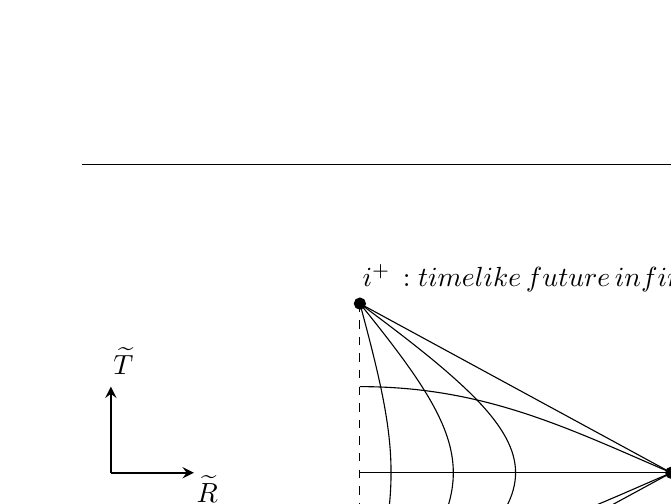
\begin{tikzpicture}[x=0.75pt,y=0.75pt,yscale=-1,xscale=1]
  %uncomment if require: \path (0,163); %set diagram left start at 0, and has height of 163
  \tikzstyle{arrow} = [thick,->,>=stealth]
  %Draw the legend on the side
 \draw [arrow] (-120,81.5) -- (-120,40);
  \draw [arrow]  (-120,81.5) -- (-80,81.5);
%Draw triangles
 \draw[dashed] (0,0) -- (0,163);
 \draw (0,0) -- (150,81.5);
  \draw (0,163) -- (150,81.5);
 %Draw Vertical curves
 \draw (0,0) .. controls (20,74) and (20,89) .. (0,163);
  \draw (0,0) .. controls (60,74) and (60,89) .. (0,163);
   \draw (0,0) .. controls (100,74) and (100,89) .. (0,163);
   %Draw Horizontal curves
     \draw (0,81.5) -- (150,81.5);
   \draw (0,40) .. controls (60,40) and (100,60) .. (150,81.5);
 \draw (0,123) .. controls (60,123) and (100,103) .. (150,81.5);
  % Label the points
  \draw  (-80,81.5)node [anchor=north west][inner sep=0.75pt]    {$\widetilde{R}$};
  \draw (-120,20) node [anchor=north west][inner sep=0.75pt]    {$ \widetilde{T}$};
  
  \draw (0,-20) node [anchor=north west][inner sep=0.75pt]    {$i^+\,:timelike \,future\, infinity$};
   \draw (0,183) node [anchor=north west][inner sep=0.75pt]    {$ i^-$};
    \draw (163,81.5) node [anchor=north west][inner sep=0.75pt]    {$i^0$};
% Draw the points
\filldraw [black] (0,0) circle (2pt);
% Draw the points
\filldraw [black] (0,163) circle (2pt);
% Draw the points
\filldraw [black] (150,81.5) circle (2pt);
  \end{tikzpicture}
  \caption{Conformal Diagram of Minkowski Space: Restricted by $|\widetilde{T}|+\widetilde{R}<\pi$ }
  \label{fig:lineup}
              \end{figure}     
  \newline
  Explain the components more. 
  \newline
  Lets look at another conformal diagram, the one for the Schwartschild Black Hole.
  In a previous class, the cruscal the convieniently had light rays at 45 degrees 
  
  \begin{figure}[!h]
               \centering
  \begin{tikzpicture}[x=0.75pt,y=0.75pt,yscale=-1,xscale=1]
  %uncomment if require: \path (0,163); %set diagram left start at 0, and has height of 163
 \draw (0,81.5) -- (0,0);
  \draw (0,81.5) -- (80,81.5);

  % Label the points
  \draw  (-20,-10)node [anchor=north west][inner sep=0.75pt]    {$\widetilde{R}$};
  \draw (90,81.5) node [anchor=north west][inner sep=0.75pt]    {$ \widetilde{T}$};

  \end{tikzpicture}
  \caption{SBH digram in cruzcal coords}
  \label{fig:lineup}
              \end{figure}  
              However, these cruzcal coordinates still need some changes to create the conformal diagram. These coordinates need to be compactified. 
              U and V are rescalings of u and v coordinates
              \begin{equation}
                 \begin{align}
                 u=t-r_* && v=t+r_* \\
                 T=\frac{V+U}{2}&&  R=\frac{V-U}{2}\\
                 U=-e^{\frac{-u}{4m}}&&V=e^{\frac{v}{4m}}\\
             \end{align}
              \end{equation}
              Define compactified coordinates
              \begin{equation}
              \begin{align}
                 V=tan\widetilde{V} && U=tan\widetilde{U}
                 \end{align}
              \end{equation}
              The same steps can be taken to transform the metric, identify a confromal factor, multiplying $d\widetilde{V}d\widetilde{U}$, then finally define new coordinates, 
              \begin{equation}
                  \widetilde{T}=\widetilde{V}+\widetilde{U}\qquad \widetilde{R}=\widetilde{V}-\widetilde{U}
              \end{equation}
              
              then get rid of conformal factor, to look at the conformally related metric. 
              \begin{equation}
                  d\widetilde{s}^2=-d\widetilde{T}^2+(function of \widetilde{T}, \widetilde{R})d\Omega^2
              \end{equation}
                \begin{figure}[!h]
               \centering
  \begin{tikzpicture}[x=0.75pt,y=0.75pt,yscale=-1,xscale=1]
  %uncomment if require: \path (0,163); %set diagram left start at 0, and has height of 163
 \tikzstyle{arrow} = [thick,->,>=stealth]
  %Draw the legend on the side
 \draw [arrow] (-120,81.5) -- (-120,40);
  \draw [arrow]  (-120,81.5) -- (-80,81.5);
  
 %Draw overly complicated geometric object 
  % Draw the points
\filldraw [black] (0,60) circle (1pt);
\filldraw [black] (171,60) circle (1pt);
\filldraw [black] (50,20) circle (1pt);
\filldraw [black] (121,20) circle (1pt);
\filldraw [black] (50,100) circle (1pt);
\filldraw [black] (121,100) circle (1pt);
  %Draw lines
  \draw (0,60) --(50,20);
  \draw (0,60)--(50,100);
  \draw (50,20)--(121,20);
  \draw (50,20)--(121,100);
  \draw (121,20)--(171,60);
   \draw (121,20)--(50,100);
   \draw (50,100)--(121,100);
   \draw (121,100)--(171,60) ;
  %Labelling
   \draw  (-80,81.5)node [anchor=north west][inner sep=0.75pt]  {$\widetilde{R}$};
  \draw (-120,20) node [anchor=north west][inner sep=0.75pt]    {$ \widetilde{T}$};
 
  \end{tikzpicture}
  \caption{Weird geometric diagram... }
  \label{fig:lineup}
              \end{figure}  
              
              
              The conformal diagram for a spherically symmetric star is \newline
               \begin{figure}[!h]
               \centering
  \begin{tikzpicture}[x=0.75pt,y=0.75pt,yscale=-1,xscale=1]
  %uncomment if require: \path (0,163); %set diagram left start at 0, and has height of 163
  \tikzstyle{arrow} = [thick,->,>=stealth]
  %Draw the legend on the side
 \draw [arrow] (-120,81.5) -- (-120,40);
  \draw [arrow]  (-120,81.5) -- (-80,81.5);
%Draw triangles
 \draw[dashed] (0,0) -- (0,163);
 \draw (0,0) -- (150,81.5);
  \draw (0,163) -- (150,81.5);
 %Draw Vertical curves
 \draw (0,0) .. controls (20,74) and (20,89) .. (0,163);
 
  
  % Label the points
  \draw  (-80,81.5)node [anchor=north west][inner sep=0.75pt]    {$\widetilde{R}$};
  \draw (-120,20) node [anchor=north west][inner sep=0.75pt]    {$ \widetilde{T}$};
  
  \draw (0,-20) node [anchor=north west][inner sep=0.75pt]    {$i^+\,:timelike \,future\, infinity$};
   \draw (0,183) node [anchor=north west][inner sep=0.75pt]    {$ i^-$};
    \draw (163,81.5) node [anchor=north west][inner sep=0.75pt]    {$i^0$};
% Draw the points
\filldraw [black] (0,0) circle (2pt);
% Draw the points
\filldraw [black] (0,163) circle (2pt);
% Draw the points
\filldraw [black] (150,81.5) circle (2pt);
  \end{tikzpicture}
  \caption{What a conformal digram will look like for our coordinates }
  \label{fig:lineup}
              \end{figure}     
              Looking at X of the digram, it looks like region I of thhe Schwatzchile Black hole. \newline If a star were to collapse to form a black hole,the following conformal diagram could describe the space.
               \begin{figure}[!h]
               \centering
  \begin{tikzpicture}[x=0.75pt,y=0.75pt,yscale=-1,xscale=1]
  %uncomment if require: \path (0,163); %set diagram left start at 0, and has height of 163
  \tikzstyle{arrow} = [thick,->,>=stealth]
  %Draw the legend on the side
 \draw [arrow] (-120,81.5) -- (-120,40);
  \draw [arrow]  (-120,81.5) -- (-80,81.5);
%Draw triangles
 \draw[dashed] (0,0) -- (0,163);
 \draw (0,0) -- (150,81.5);
  \draw (0,163) -- (150,81.5);
 %Draw Vertical curves
 \draw (0,0) .. controls (20,74) and (20,89) .. (0,163);
 
  
  % Label the points
  \draw  (-80,81.5)node [anchor=north west][inner sep=0.75pt]    {$\widetilde{R}$};
  \draw (-120,20) node [anchor=north west][inner sep=0.75pt]    {$ \widetilde{T}$};
  
  \draw (0,-20) node [anchor=north west][inner sep=0.75pt]    {$i^+$};
   \draw (0,183) node [anchor=north west][inner sep=0.75pt]    {$ i^-$};
    \draw (163,81.5) node [anchor=north west][inner sep=0.75pt]    {$i^0$};https://www.overleaf.com/project/5e95f7e972b9110001e213be
% Draw the points
\filldraw [black] (0,0) circle (2pt);
% Draw the points
\filldraw [black] (0,163) circle (2pt);
% Draw the points
\filldraw [black] (150,81.5) circle (2pt);
  \end{tikzpicture}
  \caption{What a conformal digram will look like for our coordinates }
  \label{fig:lineup}
              \end{figure}  
\end{document}